\documentclass[11pt,reqno]{amsart}

\usepackage{lmodern}
\usepackage[T1]{fontenc}
\usepackage[utf8]{inputenc}
\usepackage[english]{babel}
\usepackage{microtype}
\usepackage{amsmath,amssymb,amsthm,mathtools}
\usepackage{tikz}
\usepackage{xcolor}
\usepackage{hyperref}

\newtheorem{theorem}{Theorem}[section]
\newtheorem{proposition}[theorem]{Proposition}
\newtheorem{lemma}[theorem]{Lemma}
\newtheorem{corollary}[theorem]{Corollary}
\newtheorem{conjecture}[theorem]{Conjecture}
\newtheorem{problem}[theorem]{Problem}
\theoremstyle{definition}
\newtheorem{definition}[theorem]{Definition}
\newtheorem{remark}[theorem]{Remark}

\newcommand{\setN}{\mathbb{N}}
\newcommand{\setR}{\mathbb{R}}

\newcommand{\defin}[1]{%
\relax\ifmmode%
\textcolor{blue}{#1}%
\else \textcolor{blue}{\emph{#1}}%
\fi%
}

\newcommand{\interl}{\ll}

\title{A Planar-Network Method for Ordered Big-Block Polynomials}
\author{Per Alexandersson}
\address{Department of Mathematics, Stockholm University}
\email{per.alexandersson@math.su.se}
\date{\today}

\begin{document}

\begin{abstract}
For $j \geq 2$, let $P_{n,j}(t)$ denote the generating polynomial for set
partitions of $[n]$, weighted by the number of blocks of size at least~$j$.
These polynomials were studied in Jack Zhan's 2023 thesis, where recurrences
were derived and real-rootedness/interlacing was posed as a natural problem.
We prove real-rootedness for the ordered analog $O_{n,j}(t)$ by placing its
exact coefficient matrix inside a planar network and then applying a
Toeplitz/P\'olya-frequency argument. More generally, we show that every family
defined by a reciprocal exponential generating function of the form
\[
  \frac{1}{1-U(z)-tV(z)}
\]
with nonnegative coefficients in $U$ and $V$ is termwise real-rooted. The
ordered big-block polynomials are one instance of this template. We also
record the staircase rook interpretation for the unordered family and explain
how a stable bivariate refinement of the ordered family would imply the
corresponding unordered statement by multiplier-sequence machinery. A central
problem is to characterize when ordered recurrences admit such a planar-network
interpretation, and when this stronger structure can be upgraded to
interlacing.
\end{abstract}

\maketitle

\section{Introduction}

Let $\Pi_n$ denote the set of set partitions of $[n]=\{1,\dotsc,n\}$. For
$j \geq 2$, define
\[
  \operatorname{bb}_j(\pi)
  \coloneqq
  \#\{B \in \pi : |B| \geq j\},
\]
the number of \defin{big blocks} of~$\pi$. The associated generating
polynomial is
\[
  P_{n,j}(t)
  \coloneqq
  \sum_{\pi \in \Pi_n} t^{\operatorname{bb}_j(\pi)}.
\]

These polynomials were studied systematically in Zhan's 2023 thesis
\cite{Zhan2023}, where several recurrence formulas were obtained and the
real-rootedness and interlacing problem was highlighted. The cases $j=1$ and
$j=2$ are well behaved: $P_{n,1}(t)$ is the Touchard polynomial, while the
$j=2$ family is equivalent to the descent polynomials for run-sorted
permutations and is known to be real-rooted and interlacing
\cite{AlexanderssonNabawanda2021,BonaHezo2016,Zhan2023}.

The ordered analog turns out to be even more rigid. Let
$\Pi_n^{\operatorname{ord}}$ denote the set of ordered set partitions of
$[n]$, and define
\[
  O_{n,j}(t)
  \coloneqq
  \sum_{\pi \in \Pi_n^{\operatorname{ord}}}
  t^{\operatorname{bb}_j(\pi)}.
\]
Our main observation is that the ordered family sits inside a much broader
planar-network template. The specific ordered big-block family is then an
application of that theorem.

\medskip

For later reference, we state the ordered big-block consequence up front:

\begin{theorem}\label{thm:ordered_rr}
For every fixed $j \geq 2$ and every $n \geq 0$, the polynomial $O_{n,j}(t)$
has only real nonpositive zeros.
\end{theorem}

The remaining conjectures are:

\begin{conjecture}\label{conj:unordered_rr}
For every fixed $j \geq 2$, the polynomials $P_{n,j}(t)$ are real-rooted.
Moreover, they form a Sturm sequence:
\[
  P_{n,j}(t) \interl P_{n+1,j}(t)
  \qquad (n \geq 1).
\]
\end{conjecture}

\begin{conjecture}\label{conj:ordered_sturm}
For every fixed $j \geq 2$, the polynomials $O_{n,j}(t)$ form a Sturm
sequence:
\[
  O_{n,j}(t) \interl O_{n+1,j}(t)
  \qquad (n \geq 0).
\]
\end{conjecture}

The central structural questions of this note are the following.

\begin{problem}[Planar-network classification]\label{prob:classification}
Characterize the ordered combinatorial models, or more generally the
reciprocal generating functions and recurrences, whose exact coefficient
matrices arise as planar path matrices. The ordered big-block polynomials show
that reciprocal exponential generating functions of the form
\[
  \frac{1}{1-U(z)-tV(z)}
\]
with nonnegative coefficients in \(U\) and \(V\) form one robust class, but it
is natural to ask how far beyond this affine-linear block-weight setting the
planar-network method extends.
\end{problem}

\begin{problem}[Upgrading to Sturm sequences]\label{prob:sturm_upgrade}
Find natural hypotheses guaranteeing that a planar-network realization yields a
global interlacing theorem, rather than only termwise real-rootedness. In
particular, can one recognize when the ordered family itself forms a Sturm
sequence?
\end{problem}

\section{Touchard Polynomials and Staircase Rooks}

The \defin{Touchard polynomial} is
\[
  B_n(x)
  \coloneqq
  \sum_{k=1}^{n} S(n,k)\,x^k
  =
  \sum_{\pi \in \Pi_n} x^{\ell(\pi)},
\]
where $\ell(\pi)$ is the number of blocks of~$\pi$ and $S(n,k)$ is a
Stirling number of the second kind.

Let $\delta_{n-1}=(n-1,n-2,\dotsc,1)$ be the staircase board, and let
$R_{\delta_{n-1}}^{\mathrm{std}}(t)$ denote the ordinary staircase rook
polynomial, where nestings are allowed. Then
\[
  R_{\delta_{n-1}}^{\mathrm{std}}(t)
  =
  \sum_{k=0}^{n-1} S(n,n-k)\,t^k
  =
  t^n B_n(t^{-1}).
\]
So the ordinary staircase rook family is precisely the coefficient-reversal of
the Touchard family.

For the big-block statistic, it is convenient to reverse columns and work on
the triangular board
\[
  T_n \coloneqq \{(i,j) : 1 \leq i < j \leq n\}.
\]
If $\rho$ is a standard rook placement on $T_n$, let $D(\rho)$ be the
directed graph on $[n]$ with an edge $i \to j$ for each rook~$(i,j)$, and
define
\[
  \operatorname{rch}_j(\rho)
  \coloneqq
  \#\{\text{path components of $D(\rho)$ having at least $j$ vertices}\}.
\]

\begin{proposition}\label{prop:touchard_rook_bijection}
The map sending a standard rook placement $\rho$ on $T_n$ to the collection of
vertex sets of the path components of $D(\rho)$ is a bijection from staircase
rook placements to set partitions of $[n]$. Under this bijection, a block of
size $m$ corresponds to a path component with $m$ vertices. Consequently,
\[
  P_{n,j}(t)
  =
  \sum_{\rho} t^{\operatorname{rch}_j(\rho)},
\]
where the sum ranges over all standard rook placements $\rho$ on~$T_n$.
\end{proposition}

\begin{proof}
Because $\rho$ has at most one rook in each row and column, every vertex of
$D(\rho)$ has outdegree at most $1$ and indegree at most $1$. Since every edge
has the form $i \to j$ with $i<j$, the graph is acyclic, so every connected
component is a directed path. The vertex sets of these path components
therefore form a set partition of~$[n]$.

Conversely, if $B=\{b_1<\dotsb<b_m\}$ is a block of a set partition, place
rooks at
\[
  (b_1,b_2),\ (b_2,b_3),\ \dotsc,\ (b_{m-1},b_m).
\]
Doing this for each block produces a standard rook placement on~$T_n$, and the
two constructions are inverse to one another.
\end{proof}

\section{Unordered Big-Block Polynomials}

The following recurrence already appears in \cite[Lem.~3.2]{Zhan2023}; we
record it here because it is the basic unordered analogue of the ordered
recursions below.

\begin{proposition}\label{prop:unordered_recur}
For $n \geq 0$ and $j \geq 2$,
\begin{equation}\label{eq:unordered_recur}
  P_{n+1,j}(t)
  =
  \sum_{k=0}^{j-2} \binom{n}{k} P_{n-k,j}(t)
  + t \sum_{k=j-1}^{n} \binom{n}{k} P_{n-k,j}(t).
\end{equation}
\end{proposition}

\begin{proof}
Consider the block containing $n+1$. If it has size $k+1$, then one chooses
its other $k$ elements in $\binom{n}{k}$ ways and partitions the remaining
$n-k$ elements arbitrarily. If $k \leq j-2$, then this block is not counted by
$\operatorname{bb}_j$; if $k \geq j-1$, then it contributes an extra factor
of~$t$.
\end{proof}

Equivalently, the exponential generating function is
\begin{equation}\label{eq:unordered_egf}
  \sum_{n \geq 0} P_{n,j}(t)\,\frac{z^n}{n!}
  =
  \exp\!\left(
    \sum_{r=1}^{j-1} \frac{z^r}{r!}
    +
    t \sum_{r=j}^{\infty} \frac{z^r}{r!}
  \right).
\end{equation}

Zhan also observed that after the normalization \(Q_{n,j}(t)=tP_{n,j}(t)\), the
unordered family satisfies a derivative recurrence. For \(j=2\), this connects
the big-block polynomials to the run-sorted permutation family studied in
\cite{AlexanderssonNabawanda2021,BonaHezo2016,Zhan2023}. For \(j\ge 3\), both
real-rootedness and interlacing remain open; see
Conjecture~\ref{conj:unordered_rr}.

\section{A Planar-Network Template}

Let \(u_1,u_2,\dotsc\) and \(v_1,v_2,\dotsc\) be nonnegative real numbers, and
set
\[
  U(z)\coloneqq \sum_{r\geq 1} u_r \frac{z^r}{r!},
  \qquad
  V(z)\coloneqq \sum_{r\geq 1} v_r \frac{z^r}{r!}.
\]
Define polynomials \(W_n(t)\) by
\begin{equation}\label{eq:template_egf}
  \sum_{n \geq 0} W_n(t)\,\frac{z^n}{n!}
  =
  \frac{1}{1-U(z)-tV(z)}.
\end{equation}
Equivalently, \(W_0(t)=1\) and
\begin{equation}\label{eq:template_recur}
  W_{n+1}(t)
  =
  \sum_{r=1}^{n+1} \binom{n+1}{r}\bigl(u_r+t v_r\bigr)\,W_{n+1-r}(t).
\end{equation}
This is the natural recursion for an ordered sequence of labeled blocks, where
a block of size \(r\) carries weight \(u_r+t v_r\).

\begin{proposition}[The exact coefficient matrix is TNN]\label{prop:template_tnn}
Write
\[
  W_n(t)=\sum_{b\geq 0} M_{n,b}\,t^b,
  \qquad
  \widetilde M_{n,b}\coloneqq \frac{M_{n,b}}{n!}.
\]
Then the infinite matrix \(\widetilde M=(\widetilde M_{n,b})_{n,b\geq 0}\) is
totally nonnegative.

More precisely, \(\widetilde M\) is the transpose of the path matrix of the
planar network \(\mathcal N(U,V)\) with vertices \((x,h)\in \setN^2\), sources
\(s_b\coloneqq (0,b)\), sinks \(t_n\coloneqq (n,0)\), and edges
\[
  (x,h)\to (x+r,h)
  \quad\text{of weight}\quad
  \frac{u_r}{r!}
  \qquad (r\geq 1),
\]
and
\[
  (x,h)\to (x+r,h-1)
  \quad\text{of weight}\quad
  \frac{v_r}{r!}
  \qquad (h\geq 1,\ r\geq 1).
\]
A truncated schematic is shown in Figure~\ref{fig:template_network}.
\end{proposition}

\begin{proof}
For fixed \(b\), a path from \(s_b\) to \(t_n\) consists of arbitrary strings
of horizontal edges, separated by exactly \(b\) downward edges. Therefore the
ordinary generating function for weighted paths from \(s_b\) is
\[
  \sum_{n\geq 0} w(s_b\to t_n)\,z^n
  =
  \frac{1}{1-U(z)}
  \left(\frac{V(z)}{1-U(z)}\right)^b
  =
  \frac{V(z)^b}{(1-U(z))^{b+1}}.
\]
On the other hand, extracting the coefficient of \(t^b\) in
\eqref{eq:template_egf} gives
\[
  \sum_{n\geq 0} M_{n,b}\,\frac{z^n}{n!}
  =
  \frac{V(z)^b}{(1-U(z))^{b+1}}.
\]
Hence \(w(s_b\to t_n)=\widetilde M_{n,b}\), so the path matrix of
\(\mathcal N(U,V)\) is \((\widetilde M_{n,b})^\mathsf{T}\). Since
\(\mathcal N(U,V)\) is planar, the Lindstr\"om--Gessel--Viennot lemma
\cite{Lindstrom1973,GesselViennot1985} implies that \(\widetilde M\) is
totally nonnegative.
\end{proof}

\begin{figure}[t]
\centering
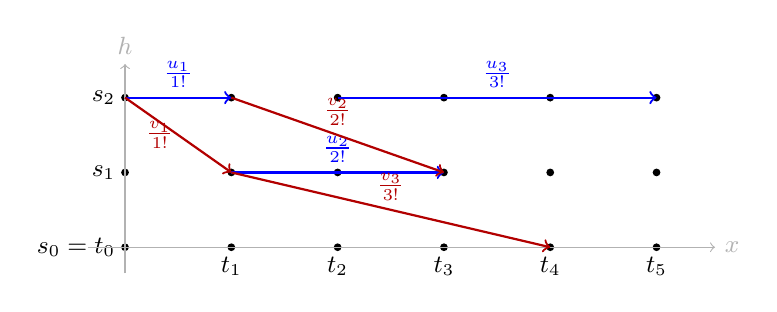
\begin{tikzpicture}[x=1.35cm,y=0.95cm, every node/.style={font=\small}]
  \foreach \x in {0,...,5} {
    \foreach \h in {0,1,2} {
      \fill (\x,\h) circle (1.4pt);
    }
  }

  \node[left] at (0,2) {$s_2$};
  \node[left] at (0,1) {$s_1$};
  \node[left] at (0,0) {$s_0=t_0$};
  \foreach \x in {1,...,5} {
    \node[below] at (\x,0) {$t_{\x}$};
  }

  \draw[gray!60,->] (-0.35,0) -- (5.55,0) node[right] {$x$};
  \draw[gray!60,->] (0,-0.35) -- (0,2.45) node[above] {$h$};

  \draw[blue,thick,->] (0,2) -- (1,2);
  \node[blue,above] at (0.5,2) {$\frac{u_1}{1!}$};

  \draw[blue,thick,->] (1,1) -- (3,1);
  \node[blue,above] at (2,1) {$\frac{u_2}{2!}$};

  \draw[blue,thick,->] (2,2) -- (5,2);
  \node[blue,above] at (3.5,2) {$\frac{u_3}{3!}$};

  \draw[red!70!black,thick,->] (0,2) -- (1,1);
  \node[red!70!black,left] at (0.55,1.5) {$\frac{v_1}{1!}$};

  \draw[red!70!black,thick,->] (1,2) -- (3,1);
  \node[red!70!black,sloped,above] at (2,1.5) {$\frac{v_2}{2!}$};

  \draw[red!70!black,thick,->] (1,1) -- (4,0);
  \node[red!70!black,sloped,above] at (2.5,0.5) {$\frac{v_3}{3!}$};
\end{tikzpicture}
\caption{A truncated schematic of the planar network \(\mathcal N(U,V)\). From
\((x,h)\) one may move horizontally to \((x+r,h)\) with weight \(u_r/r!\), or
down one level to \((x+r,h-1)\) with weight \(v_r/r!\). Only a few
representative edges are shown; all lengths \(r\geq 1\) occur.}
\label{fig:template_network}
\end{figure}

\begin{theorem}\label{thm:template_rr}
For every \(n \geq 0\), the polynomial \(W_n(t)\) has only real nonpositive
zeros.
\end{theorem}

\begin{proof}
Fix \(n\), and write
\[
  a_b \coloneqq \widetilde M_{n,b} = \frac{M_{n,b}}{n!}.
\]
Consider the strip of the network \(\mathcal N(U,V)\) between the lines
\(x=0\) and \(x=n\), with sources \(s_i\coloneqq(0,i)\) and sinks
\(u_k\coloneqq(n,k)\). Let \(T=(T_{i,k})_{i,k\geq 0}\) be its path matrix. If
\(i<k\), then \(T_{i,k}=0\), since heights never increase. If \(i\geq k\),
vertical translation by \(k\) identifies paths from \((0,i)\) to \((n,k)\)
with paths from \((0,i-k)\) to \((n,0)\), preserving all weights. Hence
\[
  T_{i,k} = a_{i-k}
  \qquad (i\geq k),
\]
so \(T\) is the lower triangular Toeplitz matrix of the sequence
\((a_0,a_1,a_2,\dotsc)\).

Because \(T\) is again a planar path matrix, it is totally nonnegative. Hence
\((a_0,a_1,a_2,\dotsc)\) is a P\'olya frequency sequence; see, for instance,
\cite[Section~4]{BrandenLeite2024x}. Since this sequence has finite support,
its generating polynomial
\[
  \sum_{b\geq 0} a_b t^b
\]
has only real nonpositive zeros. Multiplying by the positive scalar \(n!\)
does not change the zeros, so \(W_n(t)\) is real-rooted.
\end{proof}

\begin{corollary}\label{cor:ordered_big_blocks}
For fixed \(j \geq 2\), the ordered big-block polynomials satisfy
\[
  \sum_{n \geq 0} O_{n,j}(t)\,\frac{z^n}{n!}
  =
  \frac{1}{
    1
    -
    \left(
      \sum_{r=1}^{j-1} \frac{z^r}{r!}
      +
      t \sum_{r=j}^{\infty} \frac{z^r}{r!}
    \right)
  },
\]
and hence Theorem~\ref{thm:ordered_rr} holds.
Moreover,
\begin{equation}\label{eq:ordered_big_block_recur}
  O_{n+1,j}(t)
  =
  \sum_{r=1}^{j-1} \binom{n+1}{r} O_{n+1-r,j}(t)
  + t \sum_{r=j}^{n+1} \binom{n+1}{r} O_{n+1-r,j}(t).
\end{equation}
\end{corollary}

\begin{proof}
Take \(u_r=1\) and \(v_r=0\) for \(1 \leq r \leq j-1\), and \(u_r=0\),
\(v_r=1\) for \(r\geq j\). Then \eqref{eq:template_egf} becomes the ordered
big-block generating function. The recurrence \eqref{eq:ordered_big_block_recur}
is the specialization of \eqref{eq:template_recur}.
\end{proof}

\begin{remark}\label{rem:ordered_rowwise}
The proof of Theorem~\ref{thm:template_rr} is \emph{rowwise}: for each fixed
\(n\) it produces a Toeplitz totally nonnegative matrix whose first column is
the coefficient sequence of \(W_n(t)\). This is enough for real-rootedness,
but it does not yet give a single lower unitriangular totally nonnegative
matrix whose associated chain polynomials are the whole sequence
\(\{W_n(t)\}_{n\geq 0}\). Thus the interlacing theorem of
Br\"and\'en--Leite does not yet apply directly.
\end{remark}

\begin{remark}\label{rem:template_problem}
The argument above settles one broad family of examples, but it also isolates
the two guiding problems of the note. Problem~\ref{prob:classification} asks
for a structural characterization of ordered recurrences admitting a planar
network. Problem~\ref{prob:sturm_upgrade} asks how one can pass from the
rowwise totally nonnegative matrices used here to a global interlacing
statement for the whole sequence \(\{W_n(t)\}_{n\ge 0}\).
\end{remark}

\section{The Ordered-to-Unordered Bridge}

The ordered real-rootedness theorem does not by itself imply the unordered one,
but there is a natural bivariate bridge between the two families. Let
\[
  F_{n,j}(u,t)
  \coloneqq
  \sum_{\pi \in \Pi_n} u^{\ell(\pi)} t^{\operatorname{bb}_j(\pi)}
\]
and
\[
  G_{n,j}(u,t)
  \coloneqq
  \sum_{\pi \in \Pi_n^{\operatorname{ord}}}
  u^{\ell(\pi)} t^{\operatorname{bb}_j(\pi)}.
\]
If $a_{n,m,b}$ denotes the number of set partitions of $[n]$ with $m$ blocks
and exactly $b$ big blocks, then
\[
  F_{n,j}(u,t) = \sum_{m,b} a_{n,m,b}\,u^m t^b,
  \qquad
  G_{n,j}(u,t) = \sum_{m,b} m!\,a_{n,m,b}\,u^m t^b.
\]
Hence
\[
  F_{n,j}(u,t) = T_u\!\left(G_{n,j}(u,t)\right),
  \qquad
  T_u(u^m)=\frac{u^m}{m!}.
\]

\begin{remark}\label{rem:multiplier_bridge}
The sequence \(\{1/m!\}_{m\geq 0}\) is a classical multiplier sequence in the
sense of P\'olya--Schur \cite{Branden2015}. Therefore, if one could prove that
the ordered bivariate polynomials \(G_{n,j}(u,t)\) are stable, or satisfy a
sufficiently strong same-phase stability property, then applying \(T_u\) would
preserve that stability and would imply the corresponding statement for the
unordered family \(F_{n,j}(u,t)\), and in particular for
\[
  P_{n,j}(t)=F_{n,j}(1,t).
\]
This is the precise sense in which the ordered family should control the
unordered one.
\end{remark}

\section{Open Problems}

The ordered and unordered big-block families now have very different statuses.
The ordered family is termwise real-rooted by Theorem~\ref{thm:ordered_rr},
while the unordered family remains conjectural. The point of this note is that
the ordered proof is not ad hoc: it comes from an exact planar-network model
for the coefficient matrix.

This leaves two natural directions. First, one would like to solve
Problem~\ref{prob:classification} beyond the affine-linear block-weight setting
treated here. Second, one would like to solve
Problem~\ref{prob:sturm_upgrade}; a global totally nonnegative model for the
full sequence \(\{O_{n,j}(t)\}_{n\geq 0}\) would likely imply
Conjecture~\ref{conj:ordered_sturm}. Finally, a sufficiently strong stable
bivariate refinement of the ordered family would, by
Remark~\ref{rem:multiplier_bridge}, transfer to the unordered family and could
thereby prove Conjecture~\ref{conj:unordered_rr}.

\bibliographystyle{plain}
\bibliography{documents/bibliography}

\end{document}
